\chapter{مفاهیم پایه و تجهیزات‌}

در این فصل به بررسی مفاهیم و تجهیزاتی که در این پروژه استفاده شده‌است می‌پردازیم. در هر بخش دلیل انتخاب خود را شرح می‌دهیم و آن را با سایر راه‌حل‌ها مقایسه می‌کنیم.

\section{حسگر}
همانطور که گفته‌شد برای پیش‌بینی نگهداری و عمر مفید تجهیزات نیاز به نظارت و جمع‌آوری اطلاعاتی راجع‌به این تجهیزات داریم. در این پروژه، اطلاعات جمع‌آوری‌شده مربوط به وضعیت لرزش تجهیزات است که با استفاده از حسگرهای لرزش \lr{MEMS} اندازه‌گیری می‌شوند.


در این پروژه تصمیم گرفتیم که بجای دما یا رطوبت از لرزش تجهیزات برای پیش‌بینی استفاده کنیم؛ زیرا لرزش برخلاف دو معیار دیگر بطور مستقیم شرایط عملیاتی تجهیزات را منعکس می‌کند که بیشتر بر اساس رفتارهای مکانیکی مانند چرخش موتور یا حرکت جریان در لوله ایجاد می‌شوند. هم‌چنین دو معیار دیگر وابستگی زیادی به محیط دارند اما لرزش تقریبا مستقل از عوامل خارجی است\cite{jung2017vibration}.


برای اندازه‌گیری لرزش دو نوع حسگر لرزش وجود دارد. حسگرهای مبتنی بر شتاب‌سنج \lr{MEMS} بر اکثر محدودیت‌های حسگرهای قدیمی مبتنی بر شتاب‌سنج پیزوالکتریک\LTRfootnote{Piezoelectric} غلبه می‌کنند. تفاوت این دو حسگر را می‌توان در \cref{sensor_comparison} \cite{jung2017vibration} دید.

\begin{table}[h!]
  \begin{center}
    \caption{مقایسه بین دو نوع حسگر مبتنی بر پیزوالکتریک و \lr{MEMS} \cite{jung2017vibration}}
    \label{sensor_comparison}
    \begin{tabular}{|c|c|c|} % <-- Alignments: 1st column left, 2nd middle and 3rd right, with vertical lines in between
    \hline
    	& پیزوالکتریک & \lr{MEMS}\\
    	\hline
    	قیمت (دلار) & +۳۰۰ & +۱۰\\
    	\hline
    	توان مصرفی ($mW$) & ۲۷ & ۳\\
    	\hline
    	اندازه (اینچ) & ۱/۹۷ × ۰/۹۸ × ۱ & ۰/۲ × ۰/۲ × ۰/۰۵\\
    	\hline
    	تراکم نویز ($\mu g$) & ۷۰۰ & ۴۰۰۰\\
    	\hline
    	بازه شتاب ($g$) & ۱۰ & ۱۰۰\\
    	\hline
    \end{tabular}
  \end{center}
\end{table}

بطور کلی حسگرهای نوع \lr{MEMS} ارزان‌تر، کم‌مصرف‌تر و کوچک‌تر هستند. در این پروژه حسگرها با باتری کار خواهند کرد و برای اندازه‌گیری به قطعات مورد نظر متصل می‌شوند. بنابراین کم‌مصرف‌بودن، ارزانی و کوچک‌بودن برای اتصال به بدنه ویژگی‌های مطلوبی است که در حسگرهای نوع \lr{MEMS} یافت می‌شود. \cref{fig:sensor} حسگر مدل \lr{ADXL 345} که در این پروژه استفاده کرده‌ایم.

\begin{figure}[!h]
\centering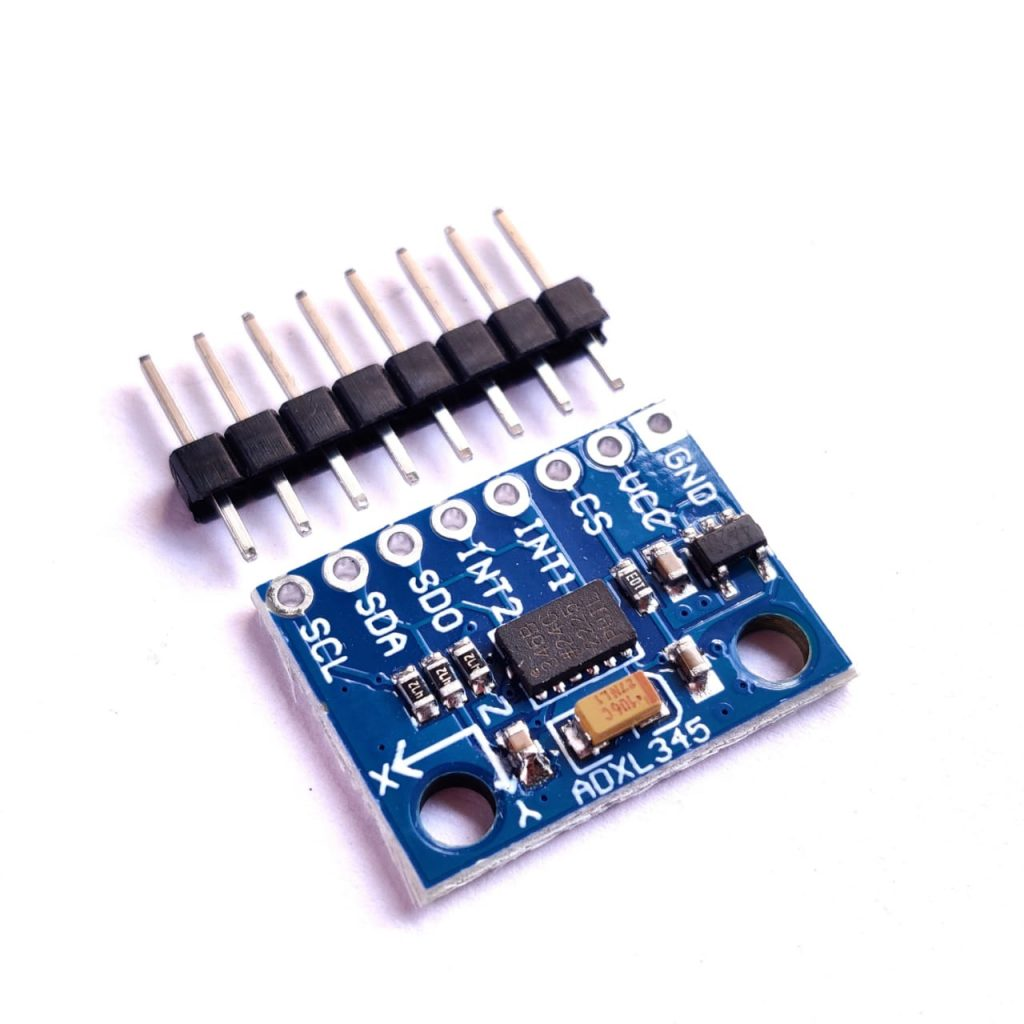
\includegraphics[scale=0.15]{sensor.png}
\caption{حسگر مدل \lr{ADXL 345}}\label{fig:sensor}
\end{figure}

این حسگر می‌تواند شتاب را در سه جهت، در چهار بازه قابل تنظیم ۲، ۴، ۸ و ۱۶ برابر گرانش با دقت‌های متفاوت اندازه‌گیری کند. خروجی این حسگر نیز با دو پروتکل \lr{SPI}\LTRfootnote{Serial Peripheral Interface} و \lr{I2C} قابل انتقال است.

\section{گره انتهایی}

برای کاهش بیشتر مصرف انرژی، دریافت اطلاعات حسگر و فرستادن آن برای دروازه به یک بورد\LTRfootnote{Board} نیاز داریم. بوردهای آردوینو\LTRfootnote{Arduino} اگرچه محدودیت‌هایی دارند، اما با توجه به ارزان‌بودن و برآورده‌کردن نیاز ما انتخاب مناسبی هستند. بورد استفاده‌شده در این پروژه آردوینو نانو است که در \cref{fig:arduino_nano} قابل‌مشاهده است. در این بورد از پورت سریال\LTRfootnote{Serial Port} برای ارتباط با ماژول زیگبی\LTRfootnote{Zigbee Module} و از پروتکل \lr{I2C} برای ارتباط با حسگر استفاده می‌کنیم. یکی از محدودیت‌های این بورد حافظه کم است که در نرخ‌های بالای نمونه‌برداری حسگر کار ما را سخت می‌کند که در فصل بعد بیشتر به آن می‌پردازیم.

\begin{figure}[!h]
\centering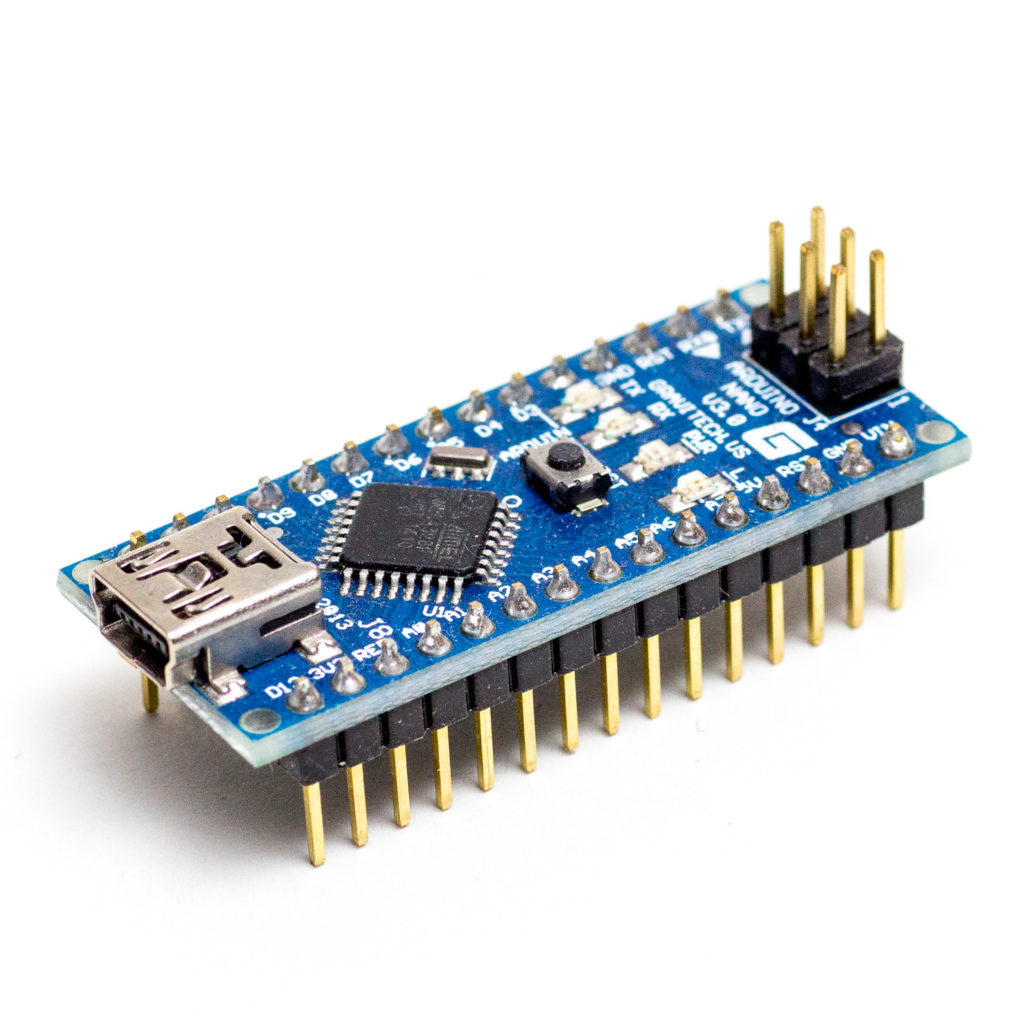
\includegraphics[scale=0.15]{arduino_nano.png}
\caption{بورد آردوینو نانو}\label{fig:arduino_nano}
\end{figure}

\section{پروتکل ارتباطی}